\documentclass[12pt]{scrartcl}
\input{../styles/Packages.tex}
% We don't need the special font encodings, but still
% good practice to include these. See:
%
% http://tex.stackexchange.com/questions/664/why-should-i-use-usepackaget1fontenc
% http://dsanta.users.ch/resources/type1.html
\usepackage[T1]{fontenc}
\usepackage{ae,aecompl}
% http://tex.stackexchange.com/a/44699
% http://tex.stackexchange.com/a/44701
\usepackage[utf8]{inputenc}

% Use Latin Modern, an improved version of the Computer Modern font
\usepackage{lmodern}

% TikZ is what lets us draw graphics
\usepackage{tikz}

% Decrease the table column spacing
% We're using tables to represent nodes in this example
\setlength{\tabcolsep}{2pt}

% Define our own macros, for convenience
%%%%%%%%%%%%%%%%%%%%%%%%%%%%%%%%%%%%%%%%%%%%%%%%%%%%%%%%%%%%%%%%%%%%%%%%%%%%%%%%

% \ensuremath{ARG} is used to enable mathematics mode in a macro
% ARG will always be rendered in math mode,
% regardless of which mode the macro is called in
%
% http://www.giss.nasa.gov/tools/latex/ensuremath.html

% These macros create single-row table with the arguments as values
% Each value is centred, and all borders are drawn
% eg \threenode{a}{b}{c} creates a single-row table with cols a, b, c

\newcommand{\onenode}[1]{%
  \begin{tabular}{|c|}
    \hline #1\\ \hline
  \end{tabular}
}
\newcommand{\twonode}[2]{%
  \begin{tabular}{|c|c|}
    \hline #1 & #2\\ \hline
  \end{tabular}
}
\newcommand{\threenode}[3]{%
  \begin{tabular}{|c|c|c|}
    \hline #1 & #2 & #3\\ \hline
  \end{tabular}
}
\newcommand{\fournode}[4]{%
  \begin{tabular}{|c|c|c|c|}
    \hline #1 & #2 & #3 & #4\\ \hline
  \end{tabular}
}
\newcommand{\fivenode}[5]{%
  \begin{tabular}{|c|c|c|c|c|}
    \hline #1 & #2 & #3 & #4 & #5\\ \hline
  \end{tabular}
}

\input{../styles/FormatAndHeader.tex}

\setcounter{sheetnr}{4} % Nummer des Übungsblattes
\setcounter{exnum}{1} % Nummer der Aufgabe

% Beginn des eigentlichen Dokuments

\begin{document}

% Aufgabe 1
\exercise{2-3-4 Suchbäume, Rot-Schwarz-Bäume}
  \begin{enumerate}
    \item Einfügen der Werte 90 und 15 in $T_{1}$
    \begin{enumerate}
      \item Einfügen des Werts 90\\
      Aufteilen des Knotens $(95, 96, 97)$, der mitteler Wert 96 nach oben ziehen.
      \begin{figure}[!h]
        \centering
        \begin{center}
          \begin{tikzpicture}
          \tikzstyle{bplus}=[rectangle split, rectangle split horizontal,rectangle split ignore empty parts,draw]
          \tikzstyle{every node}=[bplus]
          \tikzstyle{level 1}=[sibling distance=90mm]
          \tikzstyle{level 2}=[sibling distance=20mm]
          \node {55} [->]
            child {node {16 \nodepart{two} 26 \nodepart{three} 31}
              child {node {7 \nodepart{two} 13 \nodepart{three} 14}}
              child {node {19 \nodepart{two} 24}}
              child {node {28}}
              child {node {40 \nodepart{two} 44}}    
            } 
            child {node {70 \nodepart{two} 87 \nodepart{three} 96}
              child {node {59 \nodepart{two} 62}}
              child {node {77 \nodepart{two} 86}}
              child {node {95}} 
              child {node {97}} 
            };
          \end{tikzpicture}
          \end{center}
        \caption{Split $T_{1}$, Aufteilen des Knotens $(95, 96, 97)$}
        \label{fig:baum}
      \end{figure}

      Der Wert 90 wird hinzugefügt.
      \begin{figure}[!h]
        \centering
        \begin{center}
          \begin{tikzpicture}
          \tikzstyle{bplus}=[rectangle split, rectangle split horizontal,rectangle split ignore empty parts,draw]
          \tikzstyle{every node}=[bplus]
          \tikzstyle{level 1}=[sibling distance=90mm]
          \tikzstyle{level 2}=[sibling distance=20mm]
          \node {55} [->]
            child {node {16 \nodepart{two} 26 \nodepart{three} 31}
              child {node {7 \nodepart{two} 13 \nodepart{three} 14}}
              child {node {19 \nodepart{two} 24}}
              child {node {28}}
              child {node {40 \nodepart{two} 44}}    
            } 
            child {node {70 \nodepart{two} 87 \nodepart{three} 96}
              child {node {59 \nodepart{two} 62}}
              child {node {77 \nodepart{two} 86}}
              child {node {90 \nodepart{two} 95}} 
              child {node {97}} 
            };
          \end{tikzpicture}
          \end{center}
        \caption{Einfügen des Werts 90}
        \label{fig:baum}
      \end{figure}

      \item Einfügen des Werts 15\\
      Aufteilen des Knotens $(16, 26, 31)$, der mitteler Wert 26 nach oben ziehen.
      \begin{figure}[!h]
        \centering
        \begin{center}
          \begin{tikzpicture}
          \tikzstyle{bplus}=[rectangle split, rectangle split horizontal,rectangle split ignore empty parts,draw]
          \tikzstyle{every node}=[bplus]
          \tikzstyle{level 1}=[sibling distance=55mm]
          \tikzstyle{level 2}=[sibling distance=16mm]
          \node {26 \nodepart{two} 55} [->]
            child {node {16}
              child {node {7 \nodepart{two} 13 \nodepart{three} 14}}
              child {node {19 \nodepart{two} 24}}   
            }
            child {node {31}
              child {node {28}}
              child {node {40 \nodepart{two} 44}} 
            }
            child {node {70 \nodepart{two} 87 \nodepart{three} 96}
              child {node {59 \nodepart{two} 62}}
              child {node {77 \nodepart{two} 86}}
              child {node {90 \nodepart{two} 95}} 
              child {node {97}} 
            };
          \end{tikzpicture}
          \end{center}
        \caption{Aufteilen des Knotens $(16, 26, 31)$}
        \label{fig:baum}
      \end{figure}

      \newpage

      Aufteilen des Knotens $(7, 13, 14)$, der mitteler Wert 13 nach oben ziehen.
      \begin{figure}[!h]
        \centering
        \begin{center}
          \begin{tikzpicture}
          \tikzstyle{bplus}=[rectangle split, rectangle split horizontal,rectangle split ignore empty parts,draw]
          \tikzstyle{every node}=[bplus]
          \tikzstyle{level 1}=[sibling distance=55mm]
          \tikzstyle{level 2}=[sibling distance=16mm]
          \node {26 \nodepart{two} 55} [->]
            child {node {13 \nodepart{two} 16}
              child {node {7}}
              child {node {14}}
              child {node {19 \nodepart{two} 24}}   
            }
            child {node {31}
              child {node {28}}
              child {node {40 \nodepart{two} 44}} 
            }
            child {node {70 \nodepart{two} 87 \nodepart{three} 96}
              child {node {59 \nodepart{two} 62}}
              child {node {77 \nodepart{two} 86}}
              child {node {90 \nodepart{two} 95}} 
              child {node {97}} 
            };
          \end{tikzpicture}
          \end{center}
        \caption{Aufteilen des Knotens $(7, 13, 14)$}
        \label{fig:baum}
      \end{figure}

      Der Wert 15 wird hinzugefügt.
      \begin{figure}[!h]
        \centering
        \begin{center}
          \begin{tikzpicture}
          \tikzstyle{bplus}=[rectangle split, rectangle split horizontal,rectangle split ignore empty parts,draw]
          \tikzstyle{every node}=[bplus]
          \tikzstyle{level 1}=[sibling distance=55mm]
          \tikzstyle{level 2}=[sibling distance=16mm]
          \node {26 \nodepart{two} 55} [->]
            child {node {13 \nodepart{two} 16}
              child {node {7}}
              child {node {14 \nodepart{two} 15}}
              child {node {19 \nodepart{two} 24}}   
            }
            child {node {31}
              child {node {28}}
              child {node {40 \nodepart{two} 44}} 
            }
            child {node {70 \nodepart{two} 87 \nodepart{three} 96}
              child {node {59 \nodepart{two} 62}}
              child {node {77 \nodepart{two} 86}}
              child {node {90 \nodepart{two} 95}} 
              child {node {97}} 
            };
          \end{tikzpicture}
          \end{center}
        \caption{Einfügen des Werts 15}
        \label{fig:baum}
      \end{figure}

    \end{enumerate}

    \item Umwandeln des Baums $T_{1}$ in einen Rot-Schwarz-Baum
    \begin{figure}[!h]
      \centering
      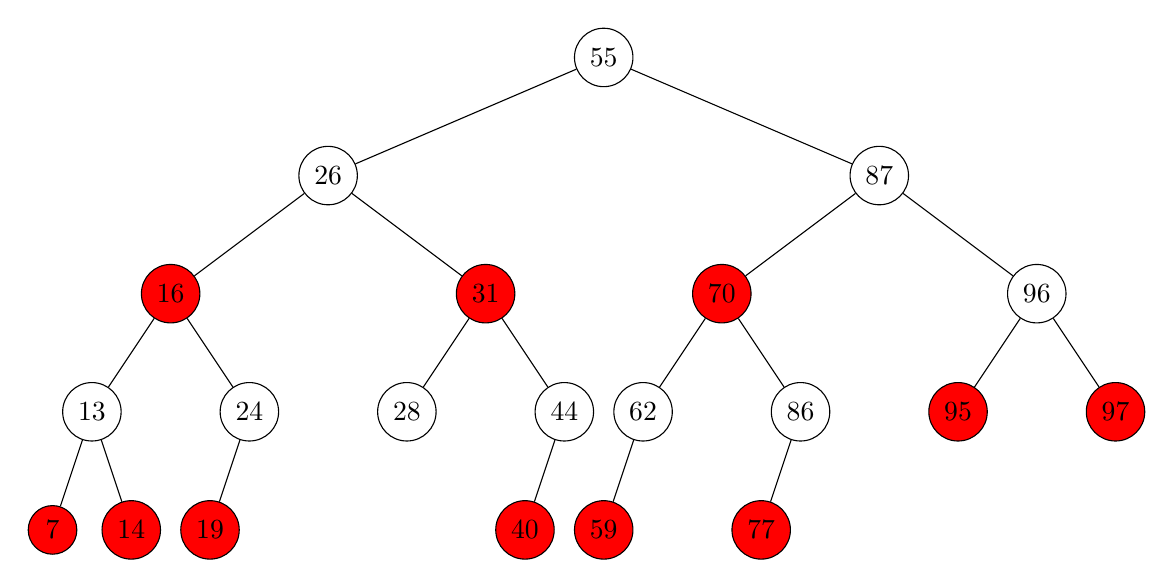
\begin{tikzpicture}
        \tikzstyle{level 1}=[sibling distance=70mm]
        \tikzstyle{level 2}=[sibling distance=40mm]
        \tikzstyle{level 3}=[sibling distance=20mm]
        \tikzstyle{level 4}=[sibling distance=10mm]
        \node[circle,draw] (a) {55}
          child {node [circle,draw] (b) {26}
            child {node [circle,draw, fill=red] (c) {16}
              child{node [circle, draw] (d) {13}
                child {node [circle, draw, fill=red] (m) {7}}
                child {node [circle, draw, fill=red] (m) {14}}
              }
              child{node [circle, draw] (d) {24}
                child {node [circle, draw, fill=red] (m) {19}}
                child[missing] {node {}}
              }
            }
            child {node [circle, draw, fill=red] (e) {31}
              child {node [circle, draw] (g) {28}}
              child {node [circle, draw] (f) {44}
                child {node [circle, draw, fill=red] (m) {40}}
                child[missing] {node {}}
              }
            }
          }
          child {node [circle, draw] (h) {87}
            child {node [circle, draw, fill=red] (i) {70}
              child {node [circle, draw] (j) {62}
                child {node [circle, draw, fill=red] (m) {59}}
                child[missing] {node {}}
              }
              child {node [circle, draw] (j) {86}
                child {node [circle, draw, fill=red] (m) {77}}
                child[missing] {node {}}
              }
            }
            child {node [circle, draw] (l) {96}
              child {node [circle, draw, fill=red] (m) {95}}
              child {node [circle, draw, fill=red] (m) {97}}
            }
          };
      \end{tikzpicture}
      \caption{Umwandeln des Baums $T_{1}$ in einen Rot-Schwarz-Baum}
      \label{fig:baum}
    \end{figure}
    
    \newpage
    \item Einfügen des Werts 4 in $T_{2}$
    \begin{figure}[!h]
      \centering
      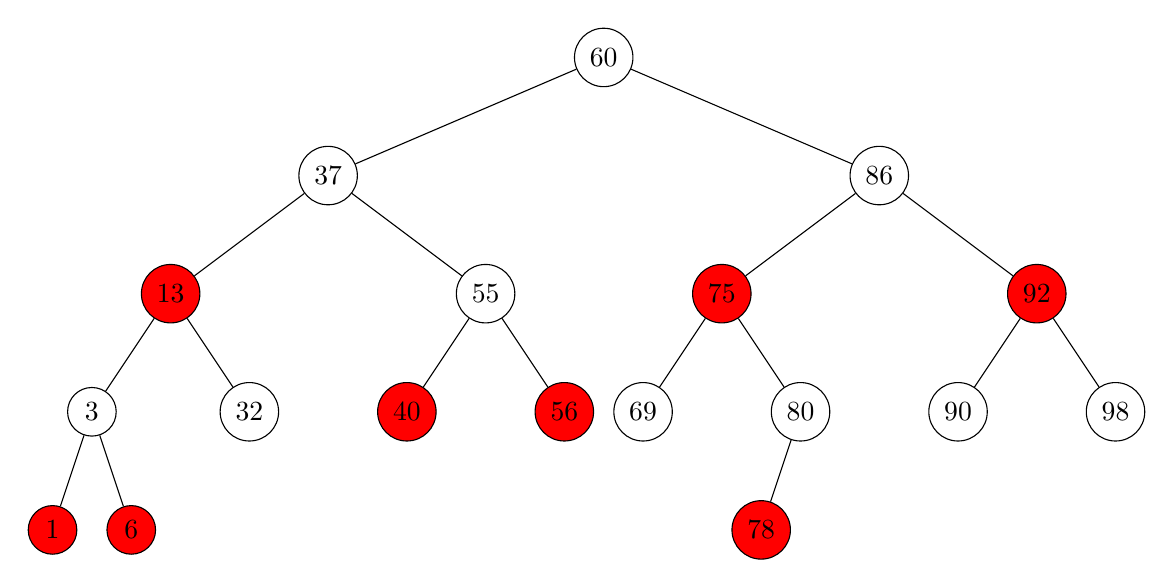
\begin{tikzpicture}
        \tikzstyle{level 1}=[sibling distance=70mm]
        \tikzstyle{level 2}=[sibling distance=40mm]
        \tikzstyle{level 3}=[sibling distance=20mm]
        \tikzstyle{level 4}=[sibling distance=10mm]
        \node[circle,draw] (a) {60}
          child {node [circle,draw] (b) {37}
            child {node [circle,draw, fill=red] (c) {13}
              child{node [circle, draw] (d) {3}
                child {node [circle, draw, fill=red] (m) {1}}
                child {node [circle, draw, fill=red] (m) {6}}
              }
              child{node [circle, draw] (d) {32}
              }
            }
            child {node [circle, draw] (e) {55}
              child {node [circle, draw, fill=red] (g) {40}}
              child {node [circle, draw, fill=red] (f) {56}}
            }
          }
          child {node [circle, draw] (h) {86}
            child {node [circle, draw, fill=red] (i) {75}
              child {node [circle, draw] (j) {69}}
              child {node [circle, draw] (j) {80}
                child {node [circle, draw, fill=red] (m) {78}}
                child[missing] {node {}}
              }
            }
            child {node [circle, draw, fill=red] (l) {92}
              child {node [circle, draw] (m) {90}}
              child {node [circle, draw] (m) {98}}
            }
          };
      \end{tikzpicture}
      \caption{$T_{2}$}
      \label{fig:baum}
    \end{figure}

    Umfärben
    \begin{figure}[!h]
      \centering
      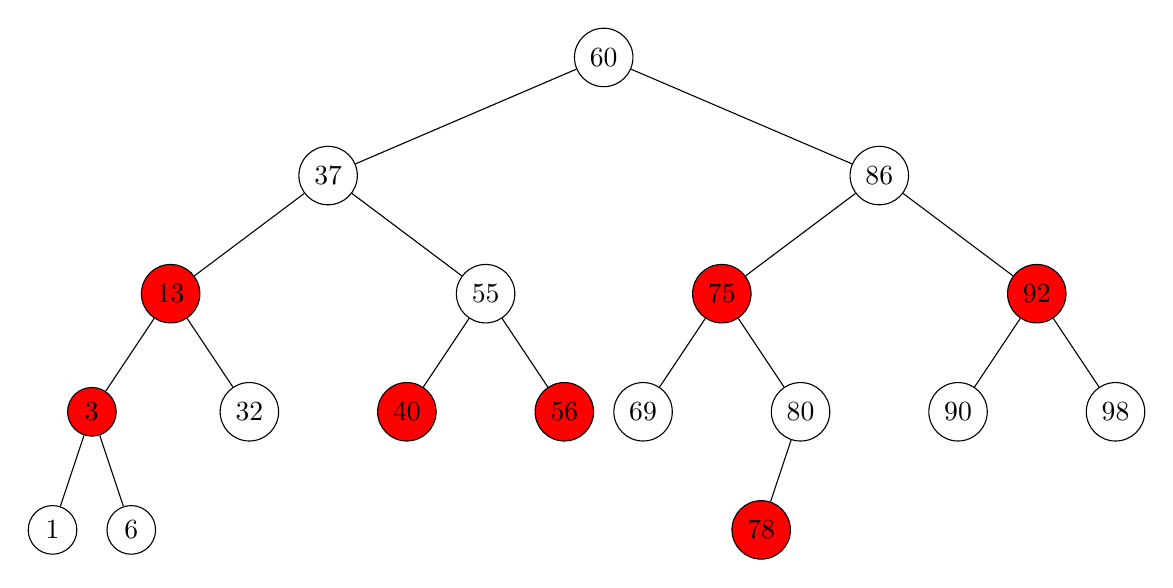
\begin{tikzpicture}
        \tikzstyle{level 1}=[sibling distance=70mm]
        \tikzstyle{level 2}=[sibling distance=40mm]
        \tikzstyle{level 3}=[sibling distance=20mm]
        \tikzstyle{level 4}=[sibling distance=10mm]
        \node[circle,draw] (a) {60}
          child {node [circle,draw] (b) {37}
            child {node [circle,draw, fill=red] (c) {13}
              child{node [circle, draw, fill=red] (d) {3}
                child {node [circle, draw] (m) {1}}
                child {node [circle, draw] (m) {6}}
              }
              child{node [circle, draw] (d) {32}
              }
            }
            child {node [circle, draw] (e) {55}
              child {node [circle, draw, fill=red] (g) {40}}
              child {node [circle, draw, fill=red] (f) {56}}
            }
          }
          child {node [circle, draw] (h) {86}
            child {node [circle, draw, fill=red] (i) {75}
              child {node [circle, draw] (j) {69}}
              child {node [circle, draw] (j) {80}
                child {node [circle, draw, fill=red] (m) {78}}
                child[missing] {node {}}
              }
            }
            child {node [circle, draw, fill=red] (l) {92}
              child {node [circle, draw] (m) {90}}
              child {node [circle, draw] (m) {98}}
            }
          };
      \end{tikzpicture}
      \caption{Umfärben}
      \label{fig:baum}
    \end{figure}

    \newpage

    Ratation
    \begin{figure}[!h]
      \centering
      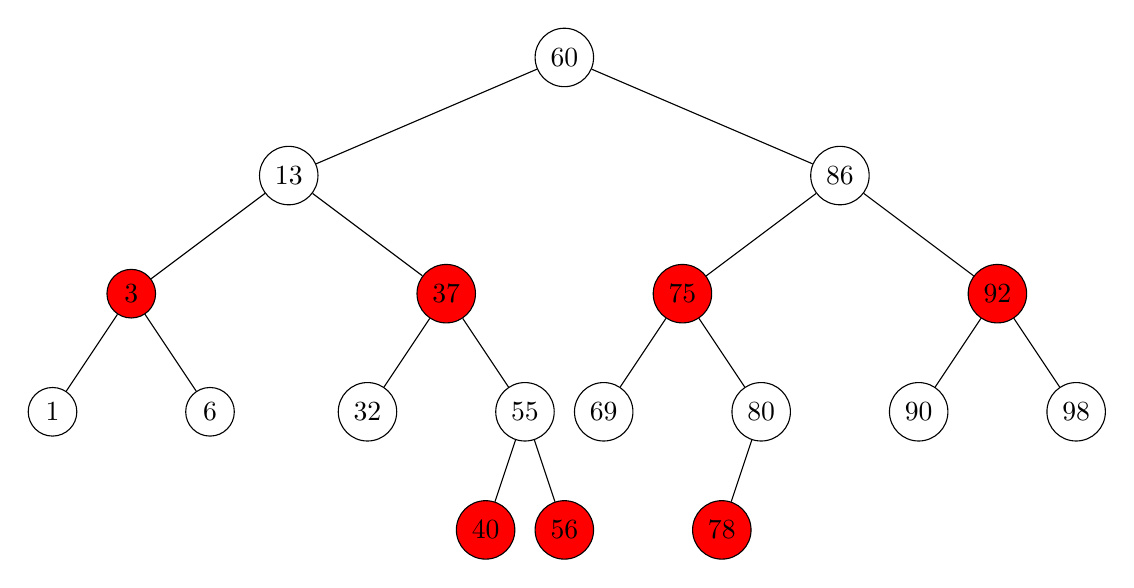
\begin{tikzpicture}
        \tikzstyle{level 1}=[sibling distance=70mm]
        \tikzstyle{level 2}=[sibling distance=40mm]
        \tikzstyle{level 3}=[sibling distance=20mm]
        \tikzstyle{level 4}=[sibling distance=10mm]
        \node[circle,draw] (a) {60}
          child {node [circle,draw] (b) {13}
            child {node [circle,draw, fill=red] (c) {3}
              child {node [circle, draw] (m) {1}}
              child {node [circle, draw] (m) {6}}
            }
            child {node [circle, draw, fill=red] (e) {37}
              child {node [circle, draw] (g) {32}}
              child {node [circle, draw] (f) {55}
                child {node [circle, draw, fill=red] (m) {40}}
                child {node [circle, draw, fill=red] (m) {56}}
              }
            }
          }
          child {node [circle, draw] (h) {86}
            child {node [circle, draw, fill=red] (i) {75}
              child {node [circle, draw] (j) {69}}
              child {node [circle, draw] (j) {80}
                child {node [circle, draw, fill=red] (m) {78}}
                child[missing] {node {}}
              }
            }
            child {node [circle, draw, fill=red] (l) {92}
              child {node [circle, draw] (m) {90}}
              child {node [circle, draw] (m) {98}}
            }
          };
      \end{tikzpicture}
      \caption{Ratation}
      \label{fig:baum}
    \end{figure}

    Einfügen von 4
    \begin{figure}[!h]
      \centering
      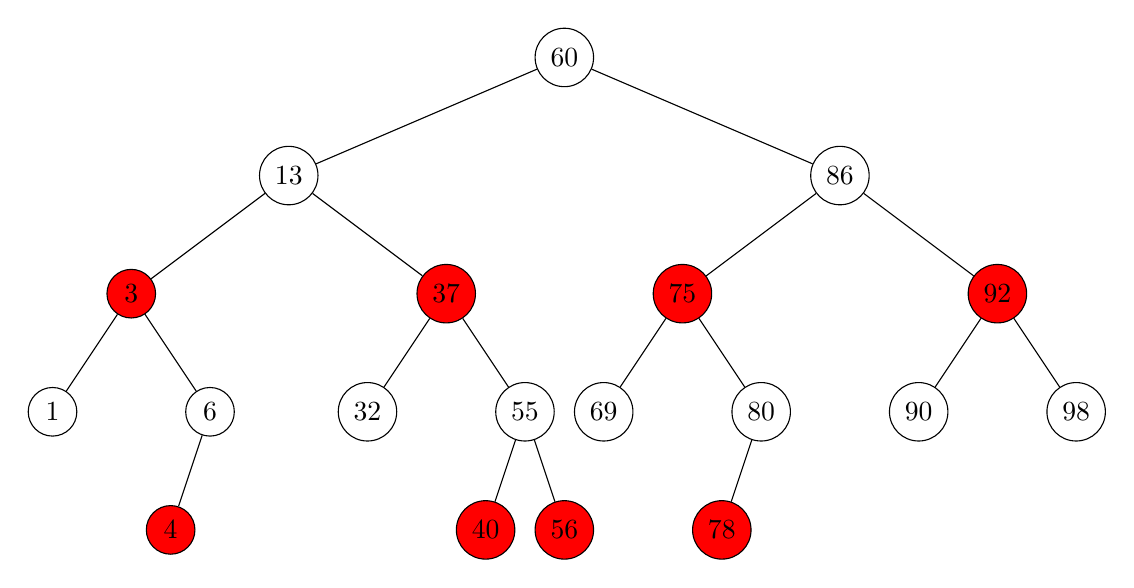
\begin{tikzpicture}
        \tikzstyle{level 1}=[sibling distance=70mm]
        \tikzstyle{level 2}=[sibling distance=40mm]
        \tikzstyle{level 3}=[sibling distance=20mm]
        \tikzstyle{level 4}=[sibling distance=10mm]
        \node[circle,draw] (a) {60}
          child {node [circle,draw] (b) {13}
            child {node [circle,draw, fill=red] (c) {3}
              child {node [circle, draw] (m) {1}}
              child {node [circle, draw] (m) {6}
                child {node [circle, draw, fill=red] (j) {4}}
                child [missing] {node {}}
              }
            }
            child {node [circle, draw, fill=red] (e) {37}
              child {node [circle, draw] (g) {32}}
              child {node [circle, draw] (f) {55}
                child {node [circle, draw, fill=red] (m) {40}}
                child {node [circle, draw, fill=red] (m) {56}}
              }
            }
          }
          child {node [circle, draw] (h) {86}
            child {node [circle, draw, fill=red] (i) {75}
              child {node [circle, draw] (j) {69}}
              child {node [circle, draw] (j) {80}
                child {node [circle, draw, fill=red] (m) {78}}
                child[missing] {node {}}
              }
            }
            child {node [circle, draw, fill=red] (l) {92}
              child {node [circle, draw] (m) {90}}
              child {node [circle, draw] (m) {98}}
            }
          };
      \end{tikzpicture}
      \caption{Einfügen von 4}
      \label{fig:baum}
    \end{figure}

  \end{enumerate}
\setcounter{exnum}{4} % Nummer der Aufgabe
\exercise{B-Bäume}
  Einfügen 88, 41, 93, 29, 7 
  \begin{center}
    % Set the options for the diagram
    % - set the distance between each level
    % - set a style for every node
    % - "bad" nodes have a 50% opaque red filling
    % - set the distances between siblings of level 1 and level 2
    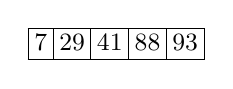
\begin{tikzpicture}[
      level distance=50pt,
      every node/.style={inner sep=0pt,font=\small},
      bad/.style={fill=red!50},
      level 1/.style={sibling distance=100pt},
      level 2/.style={sibling distance=70pt}
    ]

      % Draw the nodes, filling in their values and children
      \node {\fivenode{7}{29}{41}{88}{93}}
      ;
    \end{tikzpicture}
  \end{center}

  \newpage
  Nach dem ersten Split
  \begin{figure}[!h]
    \centering
    \begin{center}
      \begin{tikzpicture}
      \tikzstyle{bplus}=[rectangle split, rectangle split horizontal,rectangle split ignore empty parts,draw]
      \tikzstyle{every node}=[bplus]
      \tikzstyle{level 1}=[sibling distance=90mm]
      \tikzstyle{level 2}=[sibling distance=20mm]
      \node {41} [->]
            child {node {7 \nodepart{two} 29}}
            child {node {88 \nodepart{two} 93}
            };
      \end{tikzpicture}
      \end{center}
    \caption{Split $T_{1}$, Aufteilen des Knotens $(95, 96, 97)$}
    \label{fig:baum}
  \end{figure}

  Einfügen 55, 39, 14, 66, 87
  \begin{center}
    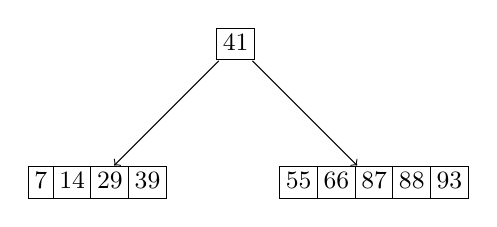
\begin{tikzpicture}[
      level distance=50pt,
      every node/.style={inner sep=0pt,font=\small},
      bad/.style={fill=red!50},
      level 1/.style={sibling distance=100pt},
      level 2/.style={sibling distance=70pt}
    ]
      \node {\onenode{41}}[->]
        child {node {\fournode{7}{14}{29}{39}}
        }
        child {node {\fivenode{55}{66}{87}{88}{93}}
        }
      ;
    \end{tikzpicture}
  \end{center}

  Nach dem zweiten Split
  \begin{center}
    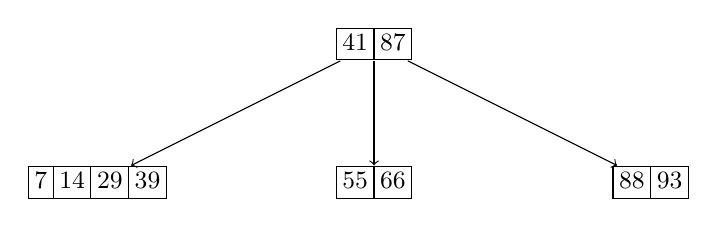
\begin{tikzpicture}[
      level distance=50pt,
      every node/.style={inner sep=0pt,font=\small},
      bad/.style={fill=red!50},
      level 1/.style={sibling distance=100pt},
      level 2/.style={sibling distance=70pt}
    ]
      \node {\twonode{41}{87}}[->]
        child {node {\fournode{7}{14}{29}{39}}
        }
        child {node {\twonode{55}{66}}
        }
        child {node {\twonode{88}{93}}
        }
      ;
    \end{tikzpicture}
  \end{center}

  Einfügen 6
  \begin{center}
    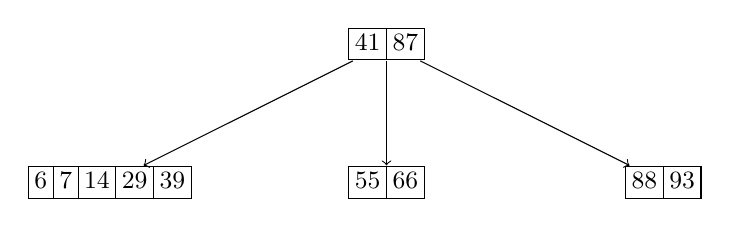
\begin{tikzpicture}[
      level distance=50pt,
      every node/.style={inner sep=0pt,font=\small},
      bad/.style={fill=red!50},
      level 1/.style={sibling distance=100pt},
      level 2/.style={sibling distance=70pt}
    ]
      \node {\twonode{41}{87}}[->]
        child {node {\fivenode{6}{7}{14}{29}{39}}
        }
        child {node {\twonode{55}{66}}
        }
        child {node {\twonode{88}{93}}
        }
      ;
    \end{tikzpicture}
  \end{center}

  Nach dem dritten Split
  \begin{center}
    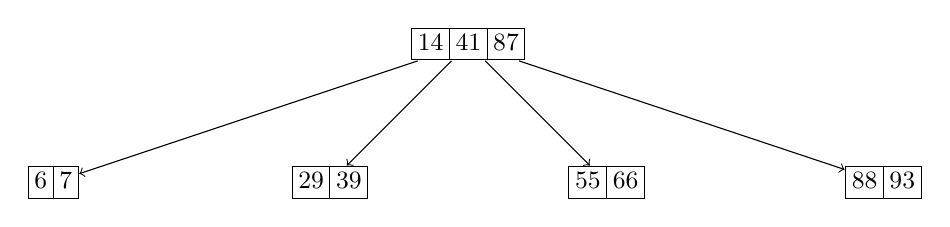
\begin{tikzpicture}[
      level distance=50pt,
      every node/.style={inner sep=0pt,font=\small},
      bad/.style={fill=red!50},
      level 1/.style={sibling distance=100pt},
      level 2/.style={sibling distance=70pt}
    ]
      \node {\threenode{14}{41}{87}}[->]
        child {node {\twonode{6}{7}}
        }
        child {node {\twonode{29}{39}}
        }
        child {node {\twonode{55}{66}}
        }
        child {node {\twonode{88}{93}}
        }
      ;
    \end{tikzpicture}
  \end{center}

  Einfügen 31, 19, 76, 71, 69
  \begin{center}
    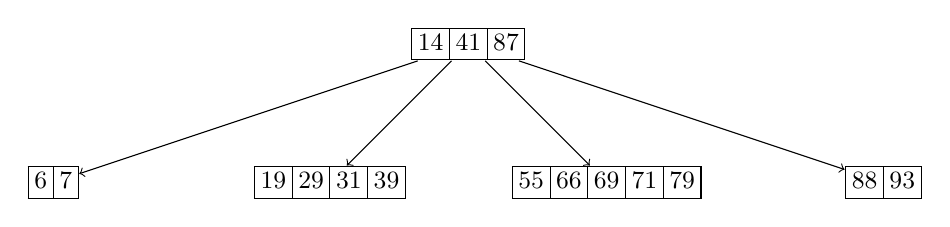
\begin{tikzpicture}[
      level distance=50pt,
      every node/.style={inner sep=0pt,font=\small},
      bad/.style={fill=red!50},
      level 1/.style={sibling distance=100pt},
      level 2/.style={sibling distance=70pt}
    ]
      \node {\threenode{14}{41}{87}}[->]
        child {node {\twonode{6}{7}}
        }
        child {node {\fournode{19}{29}{31}{39}}
        }
        child {node {\fivenode{55}{66}{69}{71}{79}}
        }
        child {node {\twonode{88}{93}}
        }
      ;
    \end{tikzpicture}
  \end{center}

  Nach dem vierten Split
  \begin{center}
    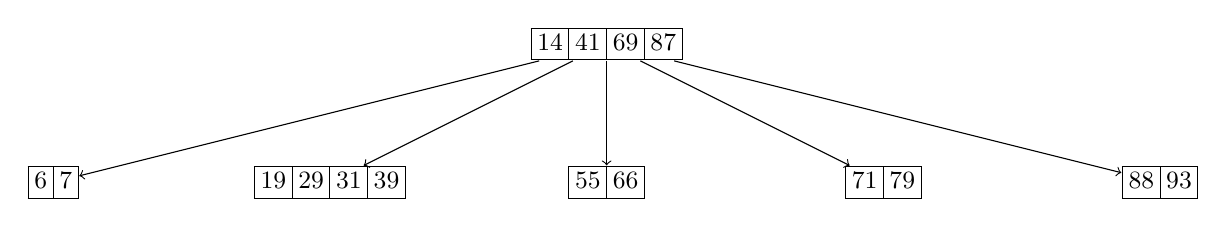
\begin{tikzpicture}[
      level distance=50pt,
      every node/.style={inner sep=0pt,font=\small},
      bad/.style={fill=red!50},
      level 1/.style={sibling distance=100pt},
      level 2/.style={sibling distance=70pt}
    ]
      \node {\fournode{14}{41}{69}{87}}[->]
        child {node {\twonode{6}{7}}
        }
        child {node {\fournode{19}{29}{31}{39}}
        }
        child {node {\twonode{55}{66}}
        }
        child {node {\twonode{71}{79}}
        }
        child {node {\twonode{88}{93}}
        }
      ;
    \end{tikzpicture}
  \end{center}

  Einfügen 24
  \begin{center}
    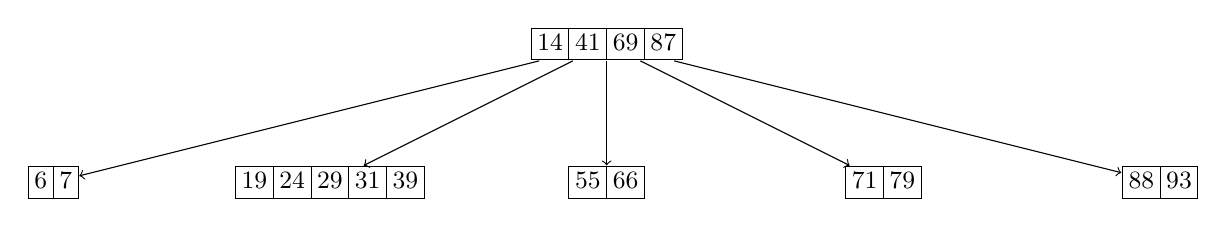
\begin{tikzpicture}[
      level distance=50pt,
      every node/.style={inner sep=0pt,font=\small},
      bad/.style={fill=red!50},
      level 1/.style={sibling distance=100pt},
      level 2/.style={sibling distance=70pt}
    ]
      \node {\fournode{14}{41}{69}{87}}[->]
        child {node {\twonode{6}{7}}
        }
        child {node {\fivenode{19}{24}{29}{31}{39}}
        }
        child {node {\twonode{55}{66}}
        }
        child {node {\twonode{71}{79}}
        }
        child {node {\twonode{88}{93}}
        }
      ;
    \end{tikzpicture}
  \end{center}

  Nach dem fünften Split
  \begin{center}
    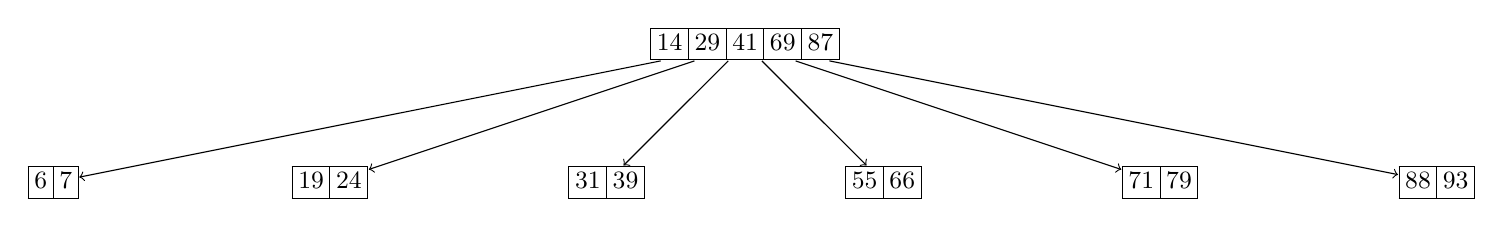
\begin{tikzpicture}[
      level distance=50pt,
      every node/.style={inner sep=0pt,font=\small},
      bad/.style={fill=red!50},
      level 1/.style={sibling distance=100pt},
      level 2/.style={sibling distance=70pt}
    ]
      \node {\fivenode{14}{29}{41}{69}{87}}[->]
        child {node {\twonode{6}{7}}
        }
        child {node {\twonode{19}{24}}
        }
        child {node {\twonode{31}{39}}
        }
        child {node {\twonode{55}{66}}
        }
        child {node {\twonode{71}{79}}
        }
        child {node {\twonode{88}{93}}
        }
      ;
    \end{tikzpicture}
  \end{center}

    Nach dem sechsten Split
    \begin{center}
      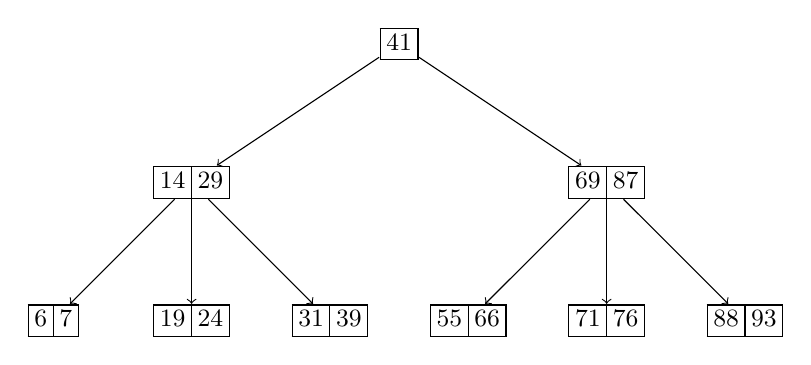
\begin{tikzpicture}[
        level distance=50pt,
        every node/.style={inner sep=0pt,font=\small},
        bad/.style={fill=red!50},
        level 1/.style={sibling distance=150pt},
        level 2/.style={sibling distance=50pt},
        level 3/.style={sibling distance=30pt},
      ]
      \node {\onenode{41}}[->]
      child {node {\twonode{14}{29}}
        child {node {\twonode{6}{7}}
        }
        child {node {\twonode{19}{24}}
        }
        child {node {\twonode{31}{39}}
        }
      }
      child {node {\twonode{69}{87}}
        child {node {\twonode{55}{66}}
        }
        child {node {\twonode{71}{76}}
        }
        child {node {\twonode{88}{93}}
        }
      };
      \end{tikzpicture}
  \end{center}
\end{document}
